\section{Resolución Problema 2} 
\subsection{Problema:}
Dada una ecuación cuadratica regresar los valores de las raíces en caso de que estén sobre el conjunto de los números reales, en caso contrario indicar que la solución esta en el conjunto de los números complejos. 

\subsection{\textbf{Descripción del problema:}}
Se debe determinar si las raíces de una ecuación cuadrática 
son reales o complejas. Si son reales, se calculan y 
se proporcionan los valores. Si son complejas, se 
indica que la solución está en el conjunto de los números complejos.

\subsection{\textbf{Definición de solución:}}
Este proyecto aborda el problema de resolver ecuaciones cuadráticas, identificando si sus raíces son reales o complejas. 
Para determinar la naturaleza de las raíces de una ecuación cuadrática de la forma  (\(ax^2 + bx + c = 0\)), se evalúa el discriminante. Si es negativo, las raíces son complejas. De lo contrario, se calculan utilizando la fórmula cuadrática estándar:

\begin{equation}
    x = \frac{-b \pm \sqrt{b^2 - 4ac}}{2a} 
    \label{eqn:formulaGeneral}
\end{equation}

Donde:
\begin{itemize}
    \item \(a\), \(b\), y \(c\) son los coeficientes de la ecuación cuadrática.
    \item El valor del discriminante determina si las raíces son reales o complejas y proporciona información sobre la cantidad de raíces distintas.
\end{itemize}


\begin{figure}[h!]
    \centering
    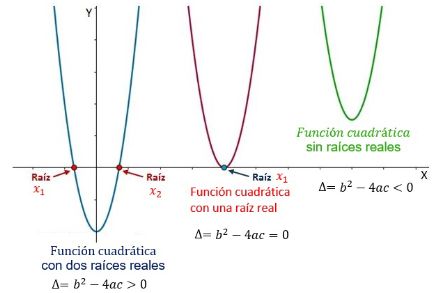
\includegraphics[width=0.6\linewidth]{./latex-imágenes/grafica_P2.png}
    \caption{Representación de la conversión}
    \label{fig: Grafica Ecuacion Recta}
\end{figure}

\subsection{\textbf{Diseño de la solución:}}

Para el diseño de la solución se seguirán los siguientes pasos:
\begin{itemize}
    \item Solicitar los coeficientes para el cálculo.
    \item Calcular el discriminante.
    \item En caso de que el discriminante sea mayor a 0, resolver la ecuación para obtener las raíces reales.
    \item En caso de que el discriminante sea igual 0, resolver la ecuación para obtener la raíz real doble.
    \item En caso de que el discriminante sea menor a 0, indicar que la solución está en el conjunto de los números complejos.
\end{itemize}

Tal y como se muestra en el siguiente diagrama de flujo.

\begin{figure}[h!]
    \centering
    \includegraphics[width = 6 cm]{./latex-imágenes/DF_problema2.jpeg}
    \caption{Diagrama de flujo del problema1}
    \label{fig:Diagramadeflujodel problema1}
\end{figure}

\subsection{\textbf{Desarrollo de la solución:}}
La implementación del código solicita al usuario los coeficientes \(a\), \(b\), y \(c\), en numeros enteros. 
\begin{javaCode}
 Scanner in= new Scanner(System.in);
        //Solicitar los datos para la formula general.
        
        System.out.println("""
                           "Ingresa los puntos a, b, c.
                           En numeros enteros.
                           Separadas por una coma(a, b, c): 
                           """);
        //Divide una cadena de texto en un arreglo de cadenas, usando la coma como separador.
        String [] datos=in.nextLine().split(",");
        //cerrar el escaneo
        in.close();
        
\end{javaCode}
Posteriormente se convierten los valores de los puntos a, b, c. En valores enteros para ser utilizados  en el calculo de la discriminante y posteriormente en la formula general.

\begin{javaCode}
    //Asigna Valores de a, b, c en enteros.
        int a= Integer.parseInt(datos[0].trim());
        int b= Integer.parseInt(datos[1].trim());
        int c= Integer.parseInt(datos[2].trim());
        
\end{javaCode}
Una vez normalizados los datos, se calcula la discriminante.
\begin{javaCode}
    //Calcula la discriminante
    double discriminante=(Math.pow(b, 2)-(4*(a*c)));
\end{javaCode}

Ya que tenemos el resultado de la discriminante, dependiendo de este se realizara la operación justa, o se dirá que la discriminante esta dentro de los números complejos.\\
Si la discriminante es mayor que cero se realiza la siguiente operación y se imprimen en pantalla los 2 posibles resultados:
\begin{javaCode}
    if (discriminante>0) {
        double x1=(-b+Math.sqrt(discriminante))/(2*a);
        double x2=(-b-Math.sqrt(discriminante))/(2*a);

        System.out.println("La raiz x1 es igual a " + x1);
        System.out.println("La raiz x1 es igual a " + x2);
            
        }
\end{javaCode}
En caso de que la discriminante sea igual a cero se realiza el siguiente calculo y se imprime el resultado en pantalla.:
\begin{javaCode}
    else if(discriminante==0){
            double x=(-b/(2*a));
            System.out.println("La raiz es igual a " + x);
        }
\end{javaCode}
Por ultimo, si la discriminante es menor a cero solo se imprimira en pantalla:\\"Esta dentro de los numeros complejos"
\begin{javaCode}
    else{
            System.out.println("Esta dentro de los numeros complejos");
        }
\end{javaCode}

\subsection{\textbf{Depuración y pruebas:}}
\begin{center}
    \begin{tabular}{|c|c|c|c|}
    \hline
    \textbf{\(a\)} & \textbf{\(b\)} & \textbf{\(c\)} & \textbf{\(Resultado\)} \\
    \hline
    1 & -3 & 2 & \(x_1 = 2, x_2 = 1\) \\
    \hline
    1 & 2 & 1 & \(x = -1\) \\
    \hline
    1 & -2 & 5 & Esta dentro de los numeros complejos\\
    \hline
    -3 & -5 & -9 & Esta dentro de los numeros complejos\\
    \hline
    \end{tabular}
    \end{center}
    
    \clearpage